% !TEX TS-program = pdflatex
% !TEX encoding = UTF-8 Unicode

% This is a simple template for a LaTeX document using the "article" class.
% See "book", "report", "letter" for other types of document.

\documentclass[11pt]{article} % use larger type; default would be 10pt
\usepackage{polski}
\usepackage{mathtools}
\usepackage{amssymb}
\usepackage{hyperref}
\usepackage[utf8]{inputenc} % set input encoding (not needed with XeLaTeX)

%%% Examples of Article customizations
% These packages are optional, depending whether you want the features they provide.
% See the LaTeX Companion or other references for full information.

%%% PAGE DIMENSIONS
\usepackage{geometry} % to change the page dimensions
\geometry{a4paper} % or letterpaper (US) or a5paper or....
% \geometry{margin=2in} % for example, change the margins to 2 inches all round
% \geometry{landscape} % set up the page for landscape
%   read geometry.pdf for detailed page layout information

\usepackage{graphicx} % support the \includegraphics command and options

% \usepackage[parfill]{parskip} % Activate to begin paragraphs with an empty line rather than an indent

%%% PACKAGES
\usepackage{booktabs} % for much better looking tables
\usepackage{array} % for better arrays (eg matrices) in maths
\usepackage{paralist} % very flexible & customisable lists (eg. enumerate/itemize, etc.)
\usepackage{verbatim} % adds environment for commenting out blocks of text & for better verbatim
\usepackage{subfig} % make it possible to include more than one captioned figure/table in a single float
% These packages are all incorporated in the memoir class to one degree or another...

%%% HEADERS & FOOTERS
\usepackage{fancyhdr} % This should be set AFTER setting up the page geometry
\pagestyle{fancy} % options: empty , plain , fancy
\renewcommand{\headrulewidth}{0pt} % customise the layout...
\lhead{}\chead{}\rhead{}
\lfoot{}\cfoot{\thepage}\rfoot{}

%%% SECTION TITLE APPEARANCE
\usepackage{sectsty}
\allsectionsfont{\sffamily\mdseries\upshape} % (See the fntguide.pdf for font help)
% (This matches ConTeXt defaults)

%%% ToC (table of contents) APPEARANCE
\usepackage[nottoc,notlof,notlot]{tocbibind} % Put the bibliography in the ToC
\usepackage[titles,subfigure]{tocloft} % Alter the style of the Table of Contents
\renewcommand{\cftsecfont}{\rmfamily\mdseries\upshape}
\renewcommand{\cftsecpagefont}{\rmfamily\mdseries\upshape} % No bold!

%%% END Article customizations

%%% The "real" document content comes below...

\title{Projekt WDWR nr 16407}
\author{Monika Pawluczuk, nr albumu 246428}

\begin{document}
\maketitle

\section{Treść zadania}

\textbf{Zagadnienie planowania produkcji}

Przedsiębiorstwo wytwarza 4 produkty: P1, P2, P3, P4 na następujących maszynach: 4 szlifierki, 2 wiertarki pionowe, 3 wiertarki poziome, 1 frezarka, 1 tokarka. 

\begin{center}
    \begin{tabular}{ | l | l | r | r | r | }
    \hline
    Narzędzie & P1 & P2 & P3 & P4 \\ \hline
    Szlifowanie & 0.4 & 0.6 & - & - \\
    Wiercenie pionowe & 0.2 & 0.1 & - & 0.6 \\
    Wiercenie poziome & 0.1 & - & 0.7 & - \\
    Frezowanie & 0.06 & 0.04 & - & 0.05 \\
    Toczenie & - & 0.05 & 0.02 & - \\ \hline
    \end{tabular}
\end{center}

\textbf{Sprzedaż produktów}
Dochody ze sprzedaży produktów (w zł/sztukę) określają składowe czterowymiarowego wektora losowego R, opisanego przez 4-wymiarowy rozkład normalny, którego wartości składowych zostały zawężone do przedziału [5,12]. Wektor wartości oczekiwanych $\ \mu $ oraz macierz kowariancji $\ \Sigma $ niezawężonego rozkładu normalnego zostały podane poniżej.

\begin{center}
$\ \mu = \begin{pmatrix}
9\\ 
9\\ 
7\\ 
6
\end{pmatrix} 
\Sigma = \begin{pmatrix}
16 & -1 & -1 & -3 \\ 
-2 & 9 & -4 & 1 \\ 
-1 & -4 & 4 & 1\\ 
-3 & -1 & 1 & 1
\end{pmatrix}$

\end{center}

\textbf{Ograniczenia rynkowe}
Istnieją ograniczenia rynkowe na liczbę sprzedawanych produktów w danym miesiącu:

\begin{center}
    \begin{tabular}{ | l | l | r | r | r | }
    \hline
    Miesiąc & P1 & P2 & P3 & P4 \\ \hline
    Styczeń & 400 & 0 & 200 & 300 \\
    Luty & 700 & 400 & 500 & 0 \\
    Marzec & 0 & 800 & 600 & 400 \\ \hline
    \end{tabular}
\end{center}

\textbf{Dodatkowe ograniczenia}
Jeżeli sprzedaż danego produktu przekracza 80\% ilości jaką może wchłonąć rynek, jego dochód spada o 20\%.

Istnieje możliwość składowania do 200 sztuk każdego produktu w danym czasie w cenie 1zł/sztukę za miesiąc. Aktualnie firma nie posiada żadnych zapasów, ale jest pożądane mieć po 50 sztuk każdego produktu pod koniec marca.

\section{Przedstawienie rozwiązania}

\subsection{Dwukryterialny model zysku i ryzyka}
W moim rozwiązaniu został zastosowany zmodyfikowany model Markowitza, maksymalizujący średni oczekiwany zysk z inwestycji $\ \mu(x)$, a minimalizujący wybraną skalarną miarę ryzyka $\ \delta(x)$,
tzn.

$\max{[ \mu(x), -\delta(x)] : x \in Q}$


W klasycznym modelu miarą ryzyka jest odchylenie standardowe, jednak znane są inne miary znajdujące lepsze zastosowania. 

W moim projekcie, zgodnie z treścią zadania, miara ta jest określona jako odchylenie przeciętne (inaczej średnie odchylenie bezwzględne), w języku angielskim znane jako MAD (Mean-Absolute Deviation).
Z definicji, jest to średnia arytmetyczna z odchyleń bezwzględnych dla wszystkich elementów zbioru danych statystycznych.

Dokładną definicję obydwu modeli oparłam na artykule naukowym "Mean-absolute deviation portfolio optimization model and its applications to Tokyo Stock Market'' z Tokyo Instuite of Technology
\footnote{
	\url{http://web.stanford.edu/class/msande348/papers/Konno_MeanAbDev_ManSciMay91.pdf}
}.

Zakładając awersję do ryzyka, w funkcji celu będziemy minimalizować ryzyko.
Funkcja celu ma zatem postać:
\begin{center}

minimize $\  E[| \sum_{j=1}^{n} R_j * x_j - E[  \sum_{j=1}^{n} R_j*x_j]  |]$

subject to $\  \sum_{j=1}^{n} E[R_j]*x_j \geqslant \rho * M_0,$

$\ \sum_{j=1}^{n} x_j = M_0,$
 
$\  0 \leqslant  x_j \leqslant  u_j, j = 1, ..., n$
\end{center}

Określając następujące definicje:
\begin{center}

$\ r_{jt} $ 
 - realizacja $\ R_j $ w czasie t (t=1,...T)

$\ r_j = E[R_j] =  \sum_{t=1}^{T} r_{jt}*1/T $

$\ a_{jt} = r_{jt} - r_j $, j=1,...,n; t=1,...,T
\end{center}

Możemy zapisać zadanie równoważnie:

\begin{center}

minimize $\   \sum_{t=1}^{T} |  \sum_{j=1}^{n} a_{jt} * x_j | * 1/T $

subject to $\  \sum_{j=1}^{n} r_j*x_j \geqslant  \rho * M_0,$

$\ \sum_{j=1}^{n} x_j = M_0,$
 
$\  0 \leqslant  x_j \leqslant  u_j, j = 1, ..., n$

\end{center}

Ze względu na to, że wartość bezwględna jest funkcją nieliniową, aby rozwiązać zadanie używając solvera CPLEX, należy przedstawić zadanie w równoważnej postaci. Dodajemy zmienną pomocniczą, którą będziemy minimalizować przy ograniczeniu jej przez przedziały w postaci szukanej przez nas funkcji. Równoważne zadanie w postaci liniowej ma postać:

\begin{center}
minimize $\   \sum_{t=1}^{T} y_t * 1/T $
 
subject to $\  y_t + \sum_{j=1}^{n} a_{jt} * x_j \geqslant 0, $ t = 1,...,T

$\  y_t - \sum_{j=1}^{n} a_{jt} * x_j \geqslant 0, $ t = 1,...,T

$\  \sum_{j=1}^{n} r_j*x_j \geqslant  \rho * M_0,$

$\ \sum_{j=1}^{n} x_j = M_0,$
 
$\  0 \leqslant  x_j \leqslant  u_j, j = 1, ..., n$
\end{center}

Dodatkowo, bazując na artykule "Stochastic Dominance Relation and Linear Programming Mean–Risk Models'' autorstwa prof. dr hab. Włodzimierza Ogryczaka, w zadaniu porgramowania liniowego \footnote{
	\url{http://www.ia.pw.edu.pl/~wogrycza/publikacje/artykuly/krakow.pdf}
} ograniczenie dotyczące zmiennej $\  y_t + \sum_{j=1}^{n} a_{jt} * x_j \geqslant 0 $ zamieniam na ograniczenie $\ y_t \geqslant 0 $ (Feinstein and Thapa, 1993).

\subsection{Macierz scenariuszy}

Próbki zostały wygenerowane na podstawie wektora wartości oczekiwanych $\ \mu $ oraz macierzy kowariancji $\ \Sigma $ w środowisku MATLAB przy użyciu funkcji mvnrnd (multivariate normal random numbers). 

\begin{center}
$\ \mu = \begin{pmatrix}
9\\ 
9\\ 
7\\ 
6
\end{pmatrix} 
\Sigma = \begin{pmatrix}
16 & -1 & -1 & -3 \\ 
-2 & 9 & -4 & 1 \\ 
-1 & -4 & 4 & 1\\ 
-3 & -1 & 1 & 1
\end{pmatrix}$

\end{center}
Wygenerowano 10.000 próbek, a następnie wybrano z nich 1000 scenariuszy, których wartości należały do przedziału [5;12]. Pozostałe scenariusze zostały odrzucone - w ten sposób nie zaburzyła się gęstość rozkładu.

Po lewej przedstawiony jest histogram wartości wygenerowanych scenariuszy bez zawężania (10 tys. próbek), po prawej histogram wartości wygenerowanych scenariuszy po zawężeniu wartości do przedziału [5; 12] (1 tys. próbek):

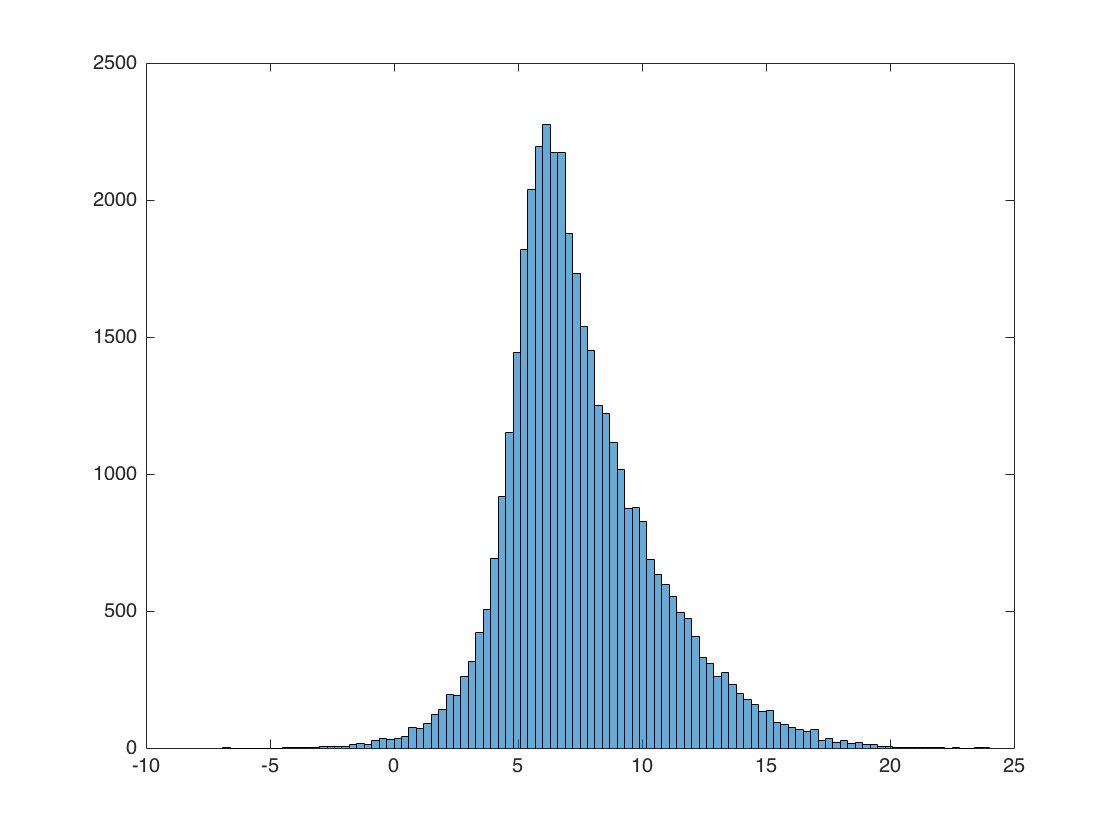
\includegraphics[width=8cm, height=8cm]{all}
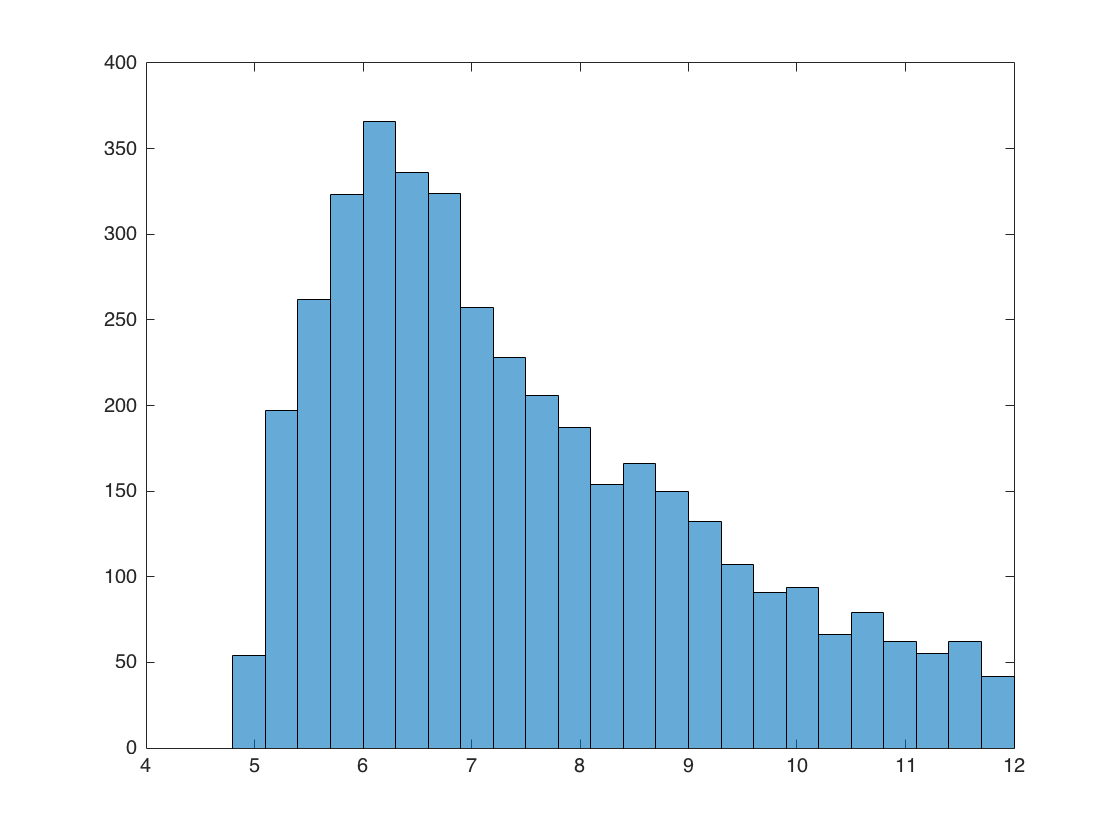
\includegraphics[width=8cm, height=8cm]{truncated}

Wygenerowane scenariusze znajdują się w pliku \emph{scenarios.dat}.

\subsection{Model}

Model został przeze mnie dopasowany na potrzeby zadania. 
\leavevmode \\

\textbf{Zdefiniowane zbiory:}

$\ PRODUCTS = \{P1, P2, P3, P4\} $ - wywtarzane przez przedsiębiorstwo produkty

$\ MONTHS = \{Jan, Feb, Mar\}  $ - miesiące dla których planujemy produkcję

$\ TOOLS = \{Szlifierka, WiertkarkaPion, WiertarkaPoz, Frezarka, Tokarka \} $ - wykorzystywane w produkcji narzędzia

$\ SCENARIOS  = \{1, ... 1000 \} $ - liczba scenariuszy
\leavevmode \\

\textbf{Parametry ustalone z treści zadania:}

$\ R\{SCENARIOS, PRODUCTS\} $ - macierz dochodów ze sprzedaży produktów (w zł/sztukę)

$\ factoryTime = 384 $  - czas pracy przedsiębiorstwa (w godzinach) w ciągu jednego miesiąca 

$\ storeFare = 1 $ - cena składowania jednej sztuki (w złotówkach) dowolnego produktu w magazynie

$\ productionTime\{TOOLS, PRODUCTS\} $ - czasy produkcji jednej sztuki danego rodzaju produktu przy użyciu danego narzędzia,
$\ p_{ij} $ to czas użycia i-tego narzędzia do produkcji j-tego produktu.  

\begin{center}
$\ productionTime = 
\begin{bmatrix}
0.4 & 0.6 & 0 &0 \\ 
0.2 & 0.1 & 0  & 0.6\\ 
 0.1& 0 & 0.7 & 0 \\ 
 0.06& 0.04 & 0 & 0.05 \\ 
 0& 0.05 & 0.02  & 0
\end{bmatrix}$
\end{center}

$ toolsNumber\{TOOLS\} $ - liczba dostępnych narzędzi danego typu w przedsiębiorstwie

\begin{center}
$\ toolsNumber = 
\begin{bmatrix}
4 \\
2 \\
3 \\
1 \\
1 \\
\end{bmatrix}$
\end{center}

$ marketLimitation\{MONTHS, PRODUCTS\} $ - ograniczenia rynkowe na liczbę sprzedawanych produktów w danym miesiącu produkcji

\begin{center}
$\ marketLimitation = 
\begin{bmatrix}
400 & 0 & 200 & 300 \\ 
700 & 400 & 500 & 0 \\
0 & 800 & 600 & 400
\end{bmatrix}$
\end{center}
\leavevmode \\

$\ prob = 1/|SCENARIOS| = 0.001 $ - prawdopodobieństwo wystąpienia scenariusza

$\ rt\{SCENARIOS, PRODUCTS\} = R_{tj} $ - realizacja scenariusza t dla produktu j

$\ r\{ PRODUCTS\} = prob *\sum_{t \in SCENARIOS} rt_{tj} $ - średni oczekiwany zysk ze sprzedaży jednej sztuki j-tego produktu 

$\ A\{SCENARIOS, PRODUCTS\} = rt_{t,j} - r_{j} $ - średnie odchylenie zysku ze sprzedaży j-tego produktu dla scenariusza t
\leavevmode \\

\textbf{Zmienne decyzyjne:}

$\ x\{MONTHS, PRODUCTS\} $ - ile produktów w danym miesiącu zostanie wyprodukowanych bezpośrednio do sprzedaży

$\ y\{MONTHS, PRODUCTS\} $ - ile produktów w danym miesiącu zostanie wyprodukowanych i przeniesionych do magazynu

$\ z\{MONTHS, PRODUCTS\} $ - ile produktów w danym miesiącu zostanie sprzedanych z magazynu

$\ abs\_sum\{MONTHS, SCENARIOS\} $ - zmienna pomocnicza do przekształcenia wartości bezwględnej 
\leavevmode \\

\textbf{Definicje ryzyka i zysku:}
\begin{center}
$\ risk = prob * \sum_{m \in MONTHS } \sum_{t \in SCENARIOS } abs\_sum_{mt} $

$\ profit = \sum_{m \in MONTHS } \sum_{j \in PRODUCTS} r_{j} * ( x_{mj} + z_{mj} - \sum_{k = 1}^{m-1} y_{kj} - z_{kj}) $
\end{center}
\leavevmode \\

\textbf{Funkcja celu minimalnego ryzyka:}

minimize $\ risk $

\textbf{Funkcja celu maksymalnego zysku:}

maximize $\ profit $
\leavevmode \\

\textbf{Ograniczenia:}
\leavevmode \\

Przekształcenie wartości bezwględnej na funkcję liniową:

$\  \sum_{j \in PRODUCTS} A_{tj} * (x_{mj} + z_{mj}) \geqslant - abs\_sum_t, 
\forall m \in MONTHS,  t \in SCENARIOS $

$\  \sum_{j \in PRODUCTS} A_{tj} * (x_{mj} + z_{mj}) \leqslant abs\_sum_t, 
\forall m \in MONTHS, t \in SCENARIOS $
\leavevmode \\

Minimalny, arbitralnie ustalony oczekiwany zysk:

$\ profit \geqslant \mu_0$
\leavevmode \\

Zmienne decyzyjne nie mogą być ujemne - nie jest możliwa ujemna produkcja produktów bezpośrednio do sprzedaży, sprzedaż produktów z magazynu ani produkcja produktów do zmagazynowania:

$\ x_{mj}, y_{mj}, z_{mj} \geqslant 0, \forall m \in MONTHS, j \in PRODUCTS $
\leavevmode \\

Nie można sprzedać więcej produktów z magazynu niż się ich znajduje w magazynie:

$\ z_{mj} \leqslant \sum_{k \in MONTHS} ^ {m-1} y_{kj} - z_{kj}, \forall m \in MONTHS, j \in PRODUCTS $
\leavevmode \\

Liczba produktów każdego rodzaju w magazynie nie może przekroczyć 200 sztuk (zakładam, że sprzedaż z magazynu odbywa się na początku miesiąca i dot. produktów zmagazynowanych w poprzednich miesiącach, a na koniec miesiąca - już po ich sprzedaży - mogę umieścić nowe produkty w magazynie):

$\ 200 \geqslant \sum_{k \in MONTHS} ^ {m-1} y_{kj} - z{kj}, \forall m \in MONTHS, j \in PRODUCTS $
\leavevmode \\

Na koniec marca przedsiębiorstwo chce mieć zmagazynowe po 50 sztuk każdego rodzaju produktu:

$\ \sum_{m \in MONTHS} y_{mj} - z_{mj} = 50, \forall  j \in PRODUCTS $
\leavevmode \\

Liczba sprzedawanych produktów, zarówno bezpośrednio z produkcji, jak i tych z magazynu nie może przekroczyć miesięcznych ograniczeń rynkowych:

$\ x_{mj} + z_{mj} \leqslant MarketLimitation_{mj}, \forall m \in MONTHS, j \in PRODUCTS $
\leavevmode \\

Sumaryczny czas na wyprodukowanie wszystkich rodzajów produktów, zarówno bezpośrednio do sprzedaży, jak i do złożenia w magazynie, nie może przekroczyć czasu w którym działa przedsiębiorstwo (24 dni robocze * 2 zmiany * 8h/zmiana) = 384 h pracy przedsiębiorstwa:

$\ \sum_{n \in TOOLS} (x_{mj} + y_{mj})*productionTime_{nj} \leqslant factoryTime, 
 \forall m \in MONTHS, j \in PRODUCTS $
\leavevmode \\

Czasy narzędzi wykorzystanych do produkcji nie mogą przekroczyć czasu w którym działa przedsiębiorstwo (zakładam, że mając kilka narzędzi tego samego typu, mogą one działać równocześnie i przez cały czas kiedy działa przedsiębiorstwo):

$\ \sum_{j \in PRODUCTS} (x_{mj} + y_{mj} * productionTime_{nj} \leqslant toolsNumber_n*factoryTime, \forall m \in MONTHS, n \in TOOLS $
\leavevmode \\

Model wraz z definicją parametrów, zmiennych i ograniczeń znajduje się w pliku \emph{Markowitz.mod}, natomiast wartości parametrów są umieszczone w pliku \emph{productionData.dat}.

\subsection{Wyznaczenie zbioru rozwiązań efektywnych w przestrzeni ryzyko-zysk}

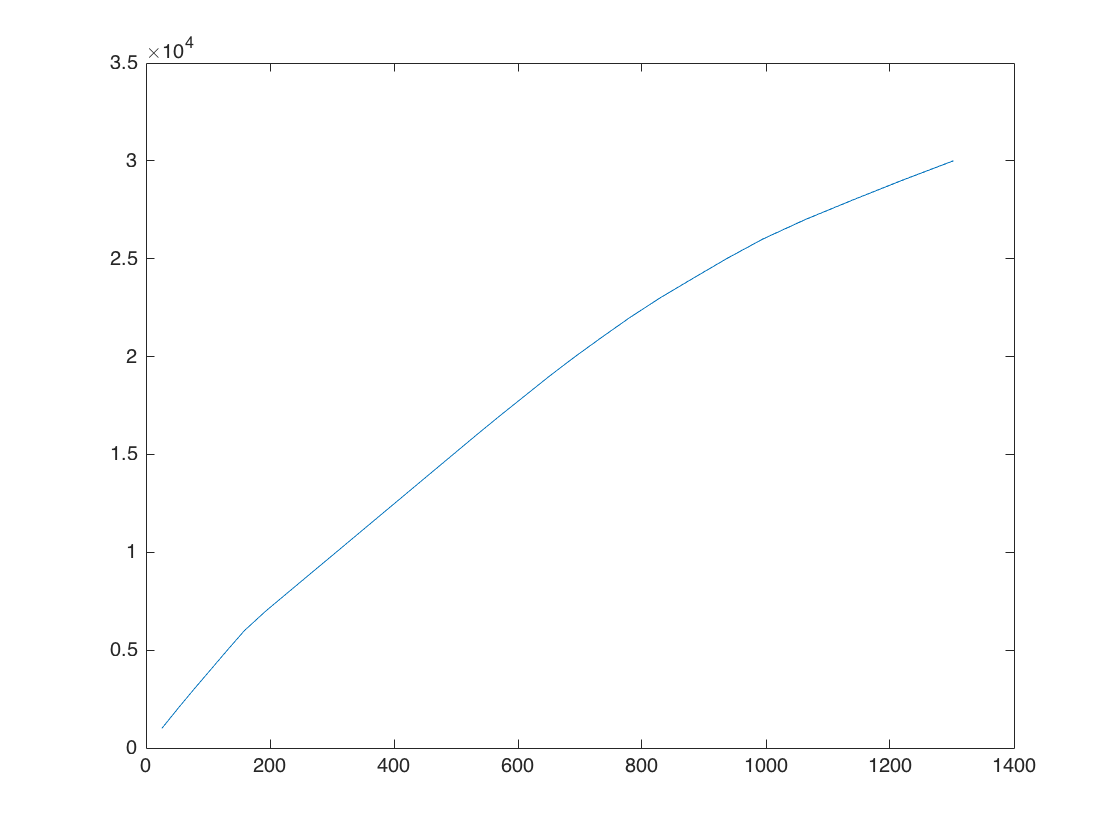
\includegraphics[width=8cm, height=8cm]{profit-risk}

\subsection{Wskazanie rozwiązań efektywnych minimalnego ryzyka i maksymalnego zysku}

\textbf{Rozwiązanie efektywne minimalnego ryzyka}

Oczekiwany maksymalny zysk: 30085.1 (zł)

Ryzyko: 1836.73

Wartości te można uzyskać przy następujących decyzjach:

\begin{center}
    \begin{tabular}{ | l | l | r | r | r | }
    \hline
    Jan & P1 &  400	& 105 	& 0 \\ \hline
    Jan & P2 &  0 		& 114 	& 0 \\ 
    Jan & P3 &  200 	& 84 	& 0 \\ 
    Jan & P4 &  300 	& 0 		& 0 \\ 
    Feb & P1 &  505 	& 0 		& 105 \\ 
    Feb & P2 &  286 	& 200 	& 114 \\
    Feb & P3 &  416 	& 117 	& 84 \\ 
    Feb & P4 &  0 		& 0 		& 0 \\ 
    Mar & P1 &  0 		& 50 	& 0 \\ 
    Mar & P2 &  486 	& 0 		& 150 \\ 
    Mar & P3 &  533 	& 0 		& 67 \\ 
    Mar & P4 &  400 	& 50 	& 0 \\  \hline
   \end{tabular}
\end{center}

\textbf{Rozwiązanie efektywne maksymalnego zysku}

Oczekiwany maksymalny zysk: 30003.8 (zł)

Ryzyko: 2047.25

\begin{center}
    \begin{tabular}{ | l | l | r | r | r | }
    \hline
    Jan & P1 &  400	& 0 	& 0 \\ \hline
    Jan & P2 &  0 		& 114 	& 0 \\ 
    Jan & P3 &  200 	& 84 	& 0 \\ 
    Jan & P4 &  300 	& 0 		& 0 \\ 
    Feb & P1 &  504 	& 0 		& 0 \\ 
    Feb & P2 &  400 	& 86 	& 0 \\
    Feb & P3 &  500 	& 33 	& 0 \\ 
    Feb & P4 &  0 		& 0 		& 0 \\ 
    Mar & P1 &  0 		& 50 	& 0 \\ 
    Mar & P2 &  486 	& 0 		& 150 \\ 
    Mar & P3 &  533 	& 0 		& 67 \\ 
    Mar & P4 &  400 	& 50 	& 0 \\  \hline
    \end{tabular}
\end{center}

Rozwiązanie efektywne minimalnego ryzyka zostało przedstawione dla mniejszej ilości próbek ze względu na ograniczenia obliczeniowe.

\subsection{Dominacja stochastyczna pomiędzy rozwiązaniami}

W dominacji stochastycznej zmienne decyzyjne są porównywane na podstawie funkcji konstruowanych z ich dystrybuant.

 Wtedy dominacja stochastyczna pierwszego rzędu (First Order Stochastic Domination, FSD) jest definiowana następująco:
 
$\ X \succeq_{FSD} Y \Leftrightarrow F_x(\eta ) \leq F_y(\eta) \forall \eta \in R $

\end{document}
